\documentclass[aspectratio=169]{beamer}

\usetheme{Madrid}
\usecolortheme{default}
\setbeamertemplate{navigation symbols}{}
\setbeamertemplate{footline}[frame number]

\usepackage[T1]{fontenc}
\usepackage{graphicx}
\usepackage{booktabs}
\usepackage{tabularx}
\usepackage{array}
\usepackage{tikz}
\usepackage{listings}
\usepackage{xcolor}

\usetikzlibrary{arrows.meta, positioning, shapes.geometric}

\graphicspath{{assets/}}

\definecolor{snistblue}{HTML}{0B4F8C}
\definecolor{snistlight}{HTML}{EAF2FB}
\definecolor{snistgold}{HTML}{D39C15}
\definecolor{softgray}{HTML}{5B6573}
\definecolor{codebg}{HTML}{F5F7FA}

\setbeamercolor{title}{fg=snistblue}
\setbeamercolor{frametitle}{fg=white, bg=snistblue}
\setbeamercolor{structure}{fg=snistblue}
\setbeamercolor{block title}{fg=white, bg=snistblue}
\setbeamercolor{block body}{bg=snistlight}
\setbeamercolor{alerted text}{fg=snistgold}

\setbeamerfont{frametitle}{series=\bfseries}
\setbeamerfont{title}{series=\bfseries}

\lstdefinestyle{pythonstyle}{
  language=Python,
  basicstyle=\ttfamily\scriptsize,
  keywordstyle=\color{snistblue}\bfseries,
  commentstyle=\color{softgray},
  backgroundcolor=\color{codebg},
  showstringspaces=false,
  frame=single,
  rulecolor=\color{snistblue},
  breaklines=true
}

\newcommand{\decktitle}{An Explainable Agentic RAG-Based Student Academic Performance Risk Assessment and Advisory System}
\newcommand{\teamshort}{Kethavath Santhosh, Jumpala Vignesh, S P S Sai Suraj}

\title[\decktitle]{\decktitle}
\subtitle{B.Tech Final Year Project Presentation}
\author[\teamshort]{
Kethavath Santhosh (22311A12P9) \\[0.15cm]
Jumpala Vignesh (22311A12P6) \\[0.15cm]
S P S Sai Suraj (22311A12N5) \\[0.35cm]
\small Under the guidance of Dr. Sunil Bhutada
}
\institute[SNIST]{
Department of Information Technology \\
Sreenidhi Institute of Science and Technology (SNIST), Hyderabad
}
\date{Academic Year 2025--2026}

\begin{document}

\begin{frame}[plain]
  \titlepage
\end{frame}

\begin{frame}{Table of Contents}
  \small
  \begin{columns}[T]
    \column{0.48\textwidth}
    \begin{enumerate}
      \item Abstract
      \item Problem Statement
      \item Introduction
      \item Existing System
      \item Proposed System
      \item Objectives
      \item Requirements
      \item Architecture Diagram
      \item UML Diagrams
      \item Modules
      \item Implementation
    \end{enumerate}
    \column{0.48\textwidth}
    \begin{enumerate}
      \setcounter{enumi}{11}
      \item Code Snippet
      \item Results / Output
      \item Advantages
      \item Limitations
      \item Conclusion
      \item Future Scope
      \item References
      \item Thank You
    \end{enumerate}
  \end{columns}
\end{frame}

\begin{frame}{Abstract}
  \begin{block}{Project Summary}
    SARS is an explainable academic support platform that converts marksheets into structured semester records, computes an interpretable risk score, and provides evidence-grounded academic advisory. The system combines Gemini vision-based extraction, user verification, database persistence, weighted risk scoring, and Retrieval-Augmented Generation in one workflow. It supports both students and faculty through dedicated dashboards for monitoring, analysis, and intervention.
  \end{block}
  \vspace{0.2cm}
  \begin{itemize}
    \item Domain: educational analytics, explainable AI, full-stack web application
    \item Core outcome: early identification of academically at-risk students
    \item Key value: transparent reasoning instead of opaque predictions
  \end{itemize}
\end{frame}

\begin{frame}{Problem Statement}
  \begin{itemize}
    \item Academic institutions store student result documents, but timely academic interpretation is still largely manual.
    \item Faculty advisors must inspect grade sheets one by one to understand CGPA, backlogs, attendance, and semester trends.
    \item Delayed interpretation causes late intervention, especially for vulnerable students.
    \item Existing workflows are not analytics-ready, scalable, or explainable.
  \end{itemize}
  \vspace{0.3cm}
  \begin{alertblock}{Need for the Project}
    A unified system is required to automatically ingest marksheets, explain academic risk clearly, and support personalized advisory and faculty intervention.
  \end{alertblock}
\end{frame}

\begin{frame}{Introduction}
  \begin{itemize}
    \item SARS belongs to the intersection of AI-assisted document processing, educational data analytics, and web-based decision support.
    \item The system targets real institutional pain points such as late risk detection, fragmented student monitoring, and generic advising.
    \item Explainability is central: the platform shows why a student is in a risk category, not just the label.
    \item Retrieval-Augmented Generation grounds advisory responses in the student's own academic record.
  \end{itemize}
  \vspace{0.2cm}
  \begin{block}{Real-World Relevance}
    The platform can help students understand their academic standing early and enable teachers to monitor cohorts more effectively.
  \end{block}
\end{frame}

\begin{frame}{Existing System}
  \begin{columns}[T]
    \column{0.56\textwidth}
    \begin{itemize}
      \item Students receive marksheets as PDF or image documents.
      \item Faculty manually read grades, backlog status, and SGPA/CGPA details.
      \item Risk interpretation depends on human effort and individual judgment.
      \item Monitoring across multiple students is repetitive and difficult to scale.
    \end{itemize}
    \column{0.40\textwidth}
    \begin{block}{Limitations}
      \begin{itemize}
        \item Time consuming
        \item Human dependency
        \item Delayed intervention
        \item No unified dashboard
        \item No explainable advisory
      \end{itemize}
    \end{block}
  \end{columns}
\end{frame}

\begin{frame}{Proposed System}
  \begin{columns}[T]
    \column{0.56\textwidth}
    \begin{itemize}
      \item Accepts marksheets in PDF or image format.
      \item Uses Gemini 2.5 Flash vision to extract academic details.
      \item Lets the user verify extracted data before persistence.
      \item Computes a weighted SARS risk score using GPA trend, backlogs, and attendance.
      \item Uses ChromaDB + Gemini based RAG for personalized advisory.
      \item Provides dedicated student and teacher dashboards.
    \end{itemize}
    \column{0.40\textwidth}
    \centering
    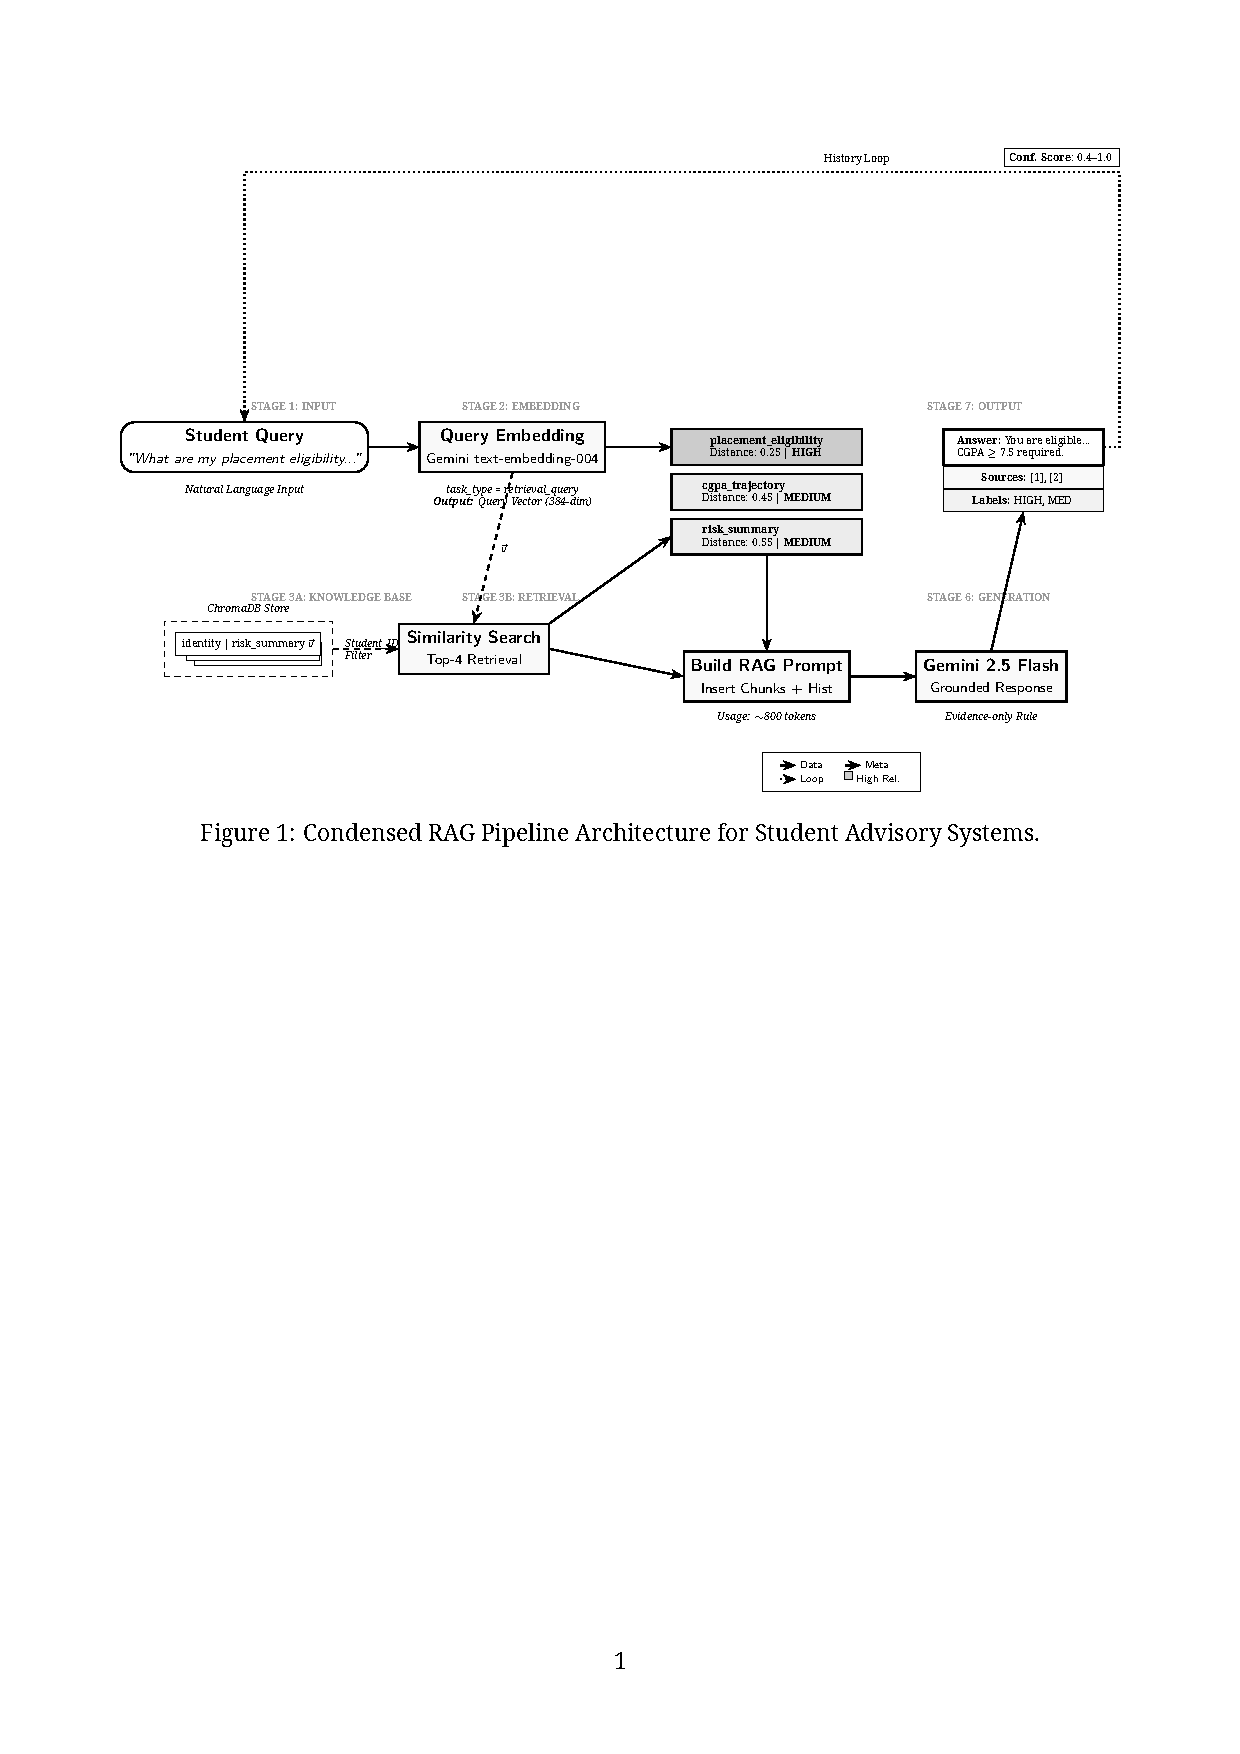
\includegraphics[width=\linewidth,height=0.68\textheight,keepaspectratio]{rag_pipeline_diagram.pdf}
  \end{columns}
\end{frame}

\begin{frame}{Objectives}
  \begin{columns}[T]
    \column{0.49\textwidth}
    \begin{block}{Functional Objectives}
      \begin{itemize}
        \item Secure login for student and teacher roles
        \item Marksheet upload and AI-assisted extraction
        \item Semester-wise academic record storage
        \item Explainable SARS score computation
        \item Personalized advisory generation
        \item Teacher-side monitoring and interventions
      \end{itemize}
    \end{block}
    \column{0.49\textwidth}
    \begin{block}{Non-Functional Objectives}
      \begin{itemize}
        \item Usability and clear dashboards
        \item Explainability and auditability
        \item Role-based security
        \item Modularity and maintainability
        \item Reliable academic data handling
      \end{itemize}
    \end{block}
  \end{columns}
\end{frame}

\begin{frame}{Requirements}
  \begin{columns}[T]
    \column{0.48\textwidth}
    \begin{block}{Hardware}
      \begin{itemize}
        \item Processor: dual-core or above
        \item RAM: minimum 8 GB
        \item Storage: 2 GB free space or above
        \item Internet: stable connection for AI APIs
      \end{itemize}
    \end{block}
    \column{0.48\textwidth}
    \begin{block}{Software}
      \begin{itemize}
        \item OS: Windows 10/11 or equivalent
        \item Frontend: React 18, JavaScript, Axios, CSS
        \item Backend: Python 3.11, FastAPI, Pydantic
        \item Database: SQLite, SQLAlchemy
        \item AI: Gemini vision, embeddings, advisory
        \item Retrieval: ChromaDB
      \end{itemize}
    \end{block}
  \end{columns}
\end{frame}

\begin{frame}{Architecture Diagram}
  \begin{columns}[T]
    \column{0.62\textwidth}
    \centering
    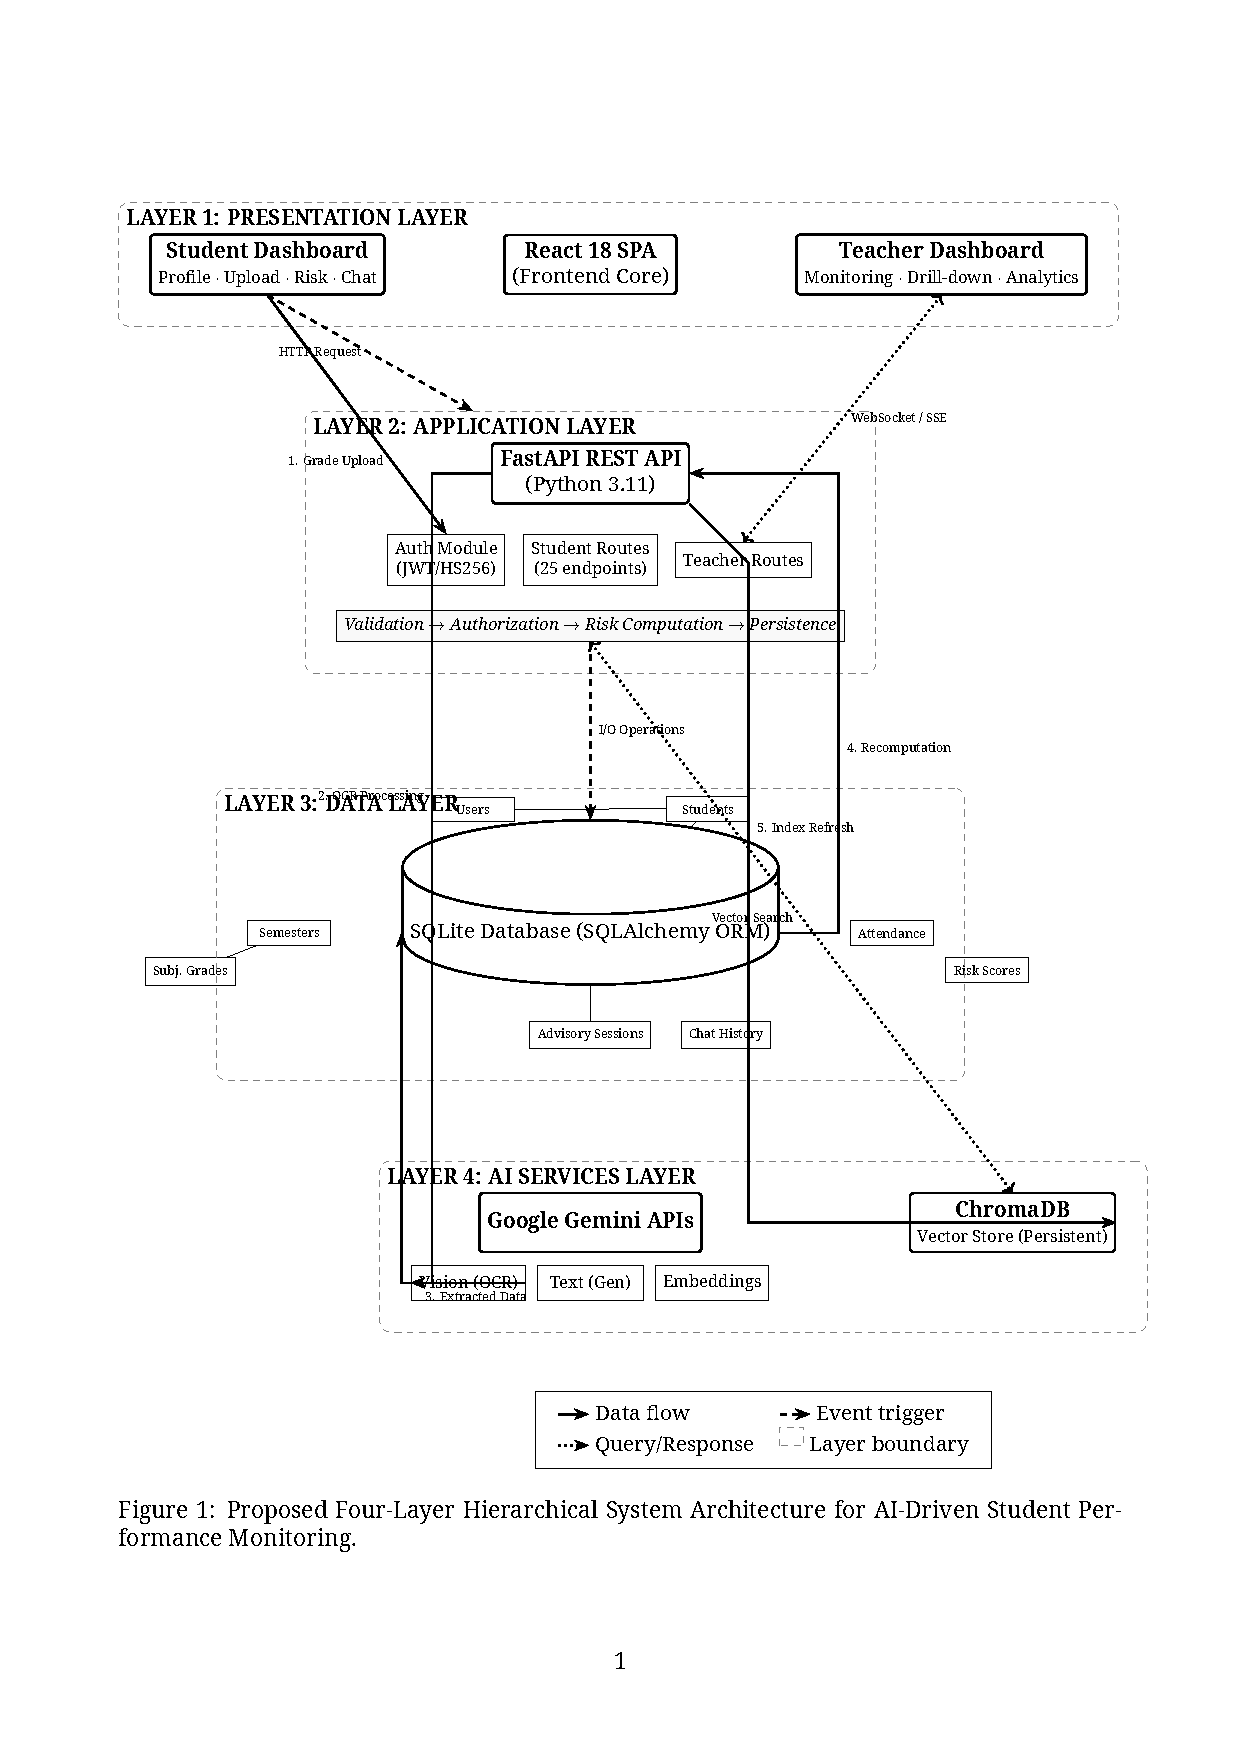
\includegraphics[width=\linewidth,height=0.73\textheight,keepaspectratio]{system_architecture_diagram.pdf}
    \column{0.34\textwidth}
    \begin{block}{Layers}
      \begin{itemize}
        \item Presentation Layer
        \item Application Layer
        \item Data Layer
        \item AI Services Layer
      \end{itemize}
    \end{block}
    \begin{block}{Flow}
      Input $\rightarrow$ Extraction $\rightarrow$ Storage $\rightarrow$ Risk Engine $\rightarrow$ Advisory / Monitoring
    \end{block}
  \end{columns}
\end{frame}

\begin{frame}{UML Diagrams}
  \begin{columns}[T]
    \column{0.49\textwidth}
    \textbf{Use Case Diagram}
    \vspace{0.15cm}
    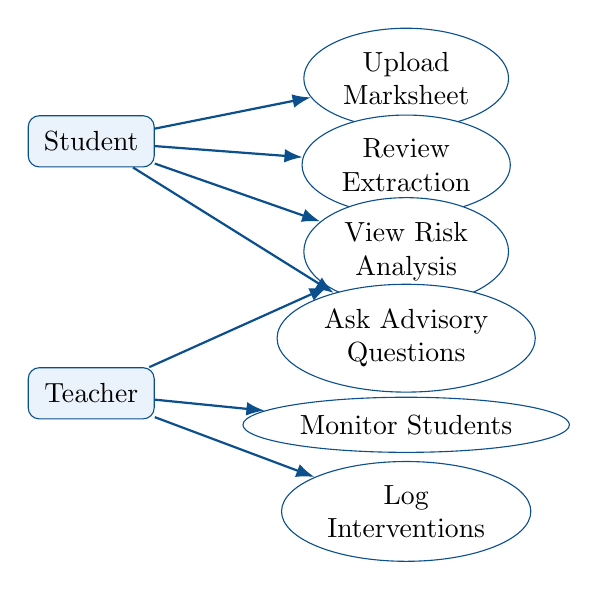
\begin{tikzpicture}[
      x=1cm, y=1cm,
      actor/.style={draw=snistblue, rounded corners, fill=snistlight, minimum width=1.6cm, minimum height=0.65cm, align=center},
      usecase/.style={draw=snistblue, ellipse, minimum width=2.6cm, minimum height=0.7cm, fill=white, align=center},
      line/.style={-Latex, thick, draw=snistblue}
    ]
      \node[actor] (student) at (0,4.2) {Student};
      \node[actor] (teacher) at (0,1.0) {Teacher};

      \node[usecase] (upload) at (4.0,5.0) {Upload\\Marksheet};
      \node[usecase] (review) at (4.0,3.9) {Review\\Extraction};
      \node[usecase] (risk) at (4.0,2.8) {View Risk\\Analysis};
      \node[usecase] (advisory) at (4.0,1.7) {Ask Advisory\\Questions};
      \node[usecase] (monitor) at (4.0,0.6) {Monitor Students};
      \node[usecase] (intervene) at (4.0,-0.5) {Log\\Interventions};

      \draw[line] (student) -- (upload);
      \draw[line] (student) -- (review);
      \draw[line] (student) -- (risk);
      \draw[line] (student) -- (advisory);
      \draw[line] (teacher) -- (monitor);
      \draw[line] (teacher) -- (intervene);
      \draw[line] (teacher) -- (risk);
    \end{tikzpicture}

    \column{0.49\textwidth}
    \textbf{Activity Diagram}
    \vspace{0.15cm}
    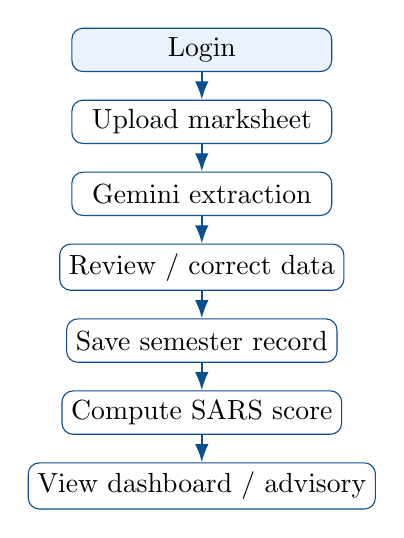
\begin{tikzpicture}[
      node distance=0.35cm,
      box/.style={draw=snistblue, rounded corners, fill=white, minimum width=3.3cm, minimum height=0.55cm, align=center},
      flow/.style={-Latex, thick, draw=snistblue}
    ]
      \node[box, fill=snistlight] (start) {Login};
      \node[box, below=of start] (upload) {Upload marksheet};
      \node[box, below=of upload] (extract) {Gemini extraction};
      \node[box, below=of extract] (review) {Review / correct data};
      \node[box, below=of review] (save) {Save semester record};
      \node[box, below=of save] (score) {Compute SARS score};
      \node[box, below=of score] (view) {View dashboard / advisory};
      \draw[flow] (start) -- (upload);
      \draw[flow] (upload) -- (extract);
      \draw[flow] (extract) -- (review);
      \draw[flow] (review) -- (save);
      \draw[flow] (save) -- (score);
      \draw[flow] (score) -- (view);
    \end{tikzpicture}
  \end{columns}
\end{frame}

\begin{frame}{Modules}
  \small
  \begin{tabularx}{\textwidth}{>{\raggedright\arraybackslash}p{0.31\textwidth}X}
    \toprule
    \textbf{Module} & \textbf{Responsibility} \\
    \midrule
    Authentication Module & Secure login, JWT token generation, role-based access control \\
    Marksheet Extraction Module & Accept PDF/image inputs and extract academic fields using Gemini vision \\
    Review and Persistence Module & Allow user verification, correction, and semester-wise data storage \\
    Risk Engine Module & Compute weighted SARS score from GPA trend, backlog count, and attendance \\
    RAG Advisory Module & Retrieve relevant academic evidence and generate personalized guidance \\
    Teacher Monitoring Module & Cohort monitoring, student drill-down, analytics, and intervention logging \\
    \bottomrule
  \end{tabularx}
\end{frame}

\begin{frame}{Implementation}
  \centering
  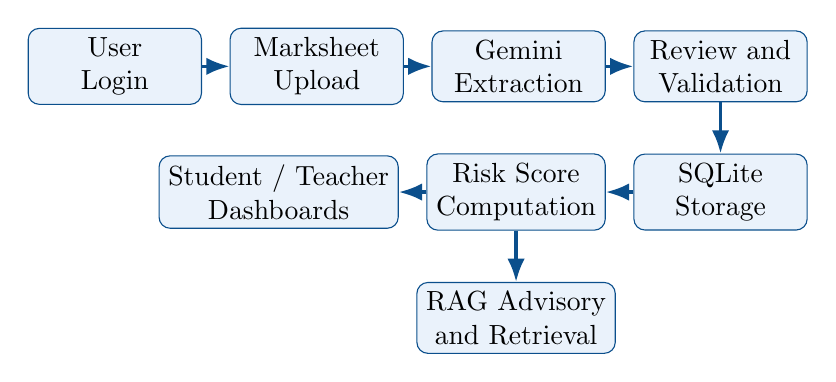
\begin{tikzpicture}[
    node distance=0.65cm and 0.35cm,
    impl/.style={draw=snistblue, rounded corners, minimum width=2.2cm, minimum height=0.9cm, align=center, fill=snistlight},
    implline/.style={-Latex, very thick, draw=snistblue}
  ]
    \node[impl] (login) {User\\Login};
    \node[impl, right=of login] (upload) {Marksheet\\Upload};
    \node[impl, right=of upload] (extract) {Gemini\\Extraction};
    \node[impl, right=of extract] (review) {Review and\\Validation};
    \node[impl, below=of review] (store) {SQLite\\Storage};
    \node[impl, left=of store] (risk) {Risk Score\\Computation};
    \node[impl, left=of risk] (view) {Student / Teacher\\Dashboards};
    \node[impl, below=of risk] (rag) {RAG Advisory\\and Retrieval};

    \draw[implline] (login) -- (upload);
    \draw[implline] (upload) -- (extract);
    \draw[implline] (extract) -- (review);
    \draw[implline] (review) -- (store);
    \draw[implline] (store) -- (risk);
    \draw[implline] (risk) -- (view);
    \draw[implline] (risk) -- (rag);
  \end{tikzpicture}
  \vspace{0.35cm}
  \begin{itemize}
    \item Backend implemented with FastAPI and SQLAlchemy
    \item Frontend implemented with React dashboards for both student and teacher users
    \item RAG indexing uses ChromaDB for student-scoped retrieval
  \end{itemize}
\end{frame}

\begin{frame}[fragile]{Code Snippet}
  \begin{lstlisting}[style=pythonstyle]
gpa_component = round(gpa_risk * 0.40, 4)
backlog_component = round(backlog_risk * 0.35, 4)
attendance_component = round(attendance_risk * 0.25, 4)

sars_score = round(
    gpa_component + backlog_component + attendance_component, 2
)

if sars_score < 25.0:
    risk_level = "LOW"
elif sars_score < 50.0:
    risk_level = "WATCH"
elif sars_score < 75.0:
    risk_level = "MODERATE"
else:
    risk_level = "HIGH"
  \end{lstlisting}
  \vspace{0.1cm}
  \begin{itemize}
    \item The risk score is transparent because each factor contributes a known weight.
    \item Risk levels are easy to interpret for both students and faculty.
  \end{itemize}
\end{frame}

\begin{frame}{Results / Output}
  \scriptsize
  \begin{columns}[T]
    \column{0.56\textwidth}
    \begin{tabularx}{\linewidth}{>{\raggedright\arraybackslash}p{0.45\linewidth}X}
      \toprule
      \textbf{Metric} & \textbf{Verified Result} \\
      \midrule
      Extraction accuracy & 66 / 66 subjects extracted across 7 semesters (100\%) \\
      CGPA validation & Weighted CGPA 8.55 matched official 8.55 \\
      Risk coverage & Demo cohort covered Low, Watch, Moderate, and High categories \\
      Token efficiency & RAG reduced request tokens from about 3000 to about 800 \\
      Capacity gain & About 73\% token reduction and 3.75x estimated capacity improvement \\
      \bottomrule
    \end{tabularx}
    \vspace{0.2cm}
    \begin{itemize}
      \item Output screens demonstrate upload, risk visualization, advisory, and teacher analytics.
    \end{itemize}
    \column{0.40\textwidth}
    \centering
    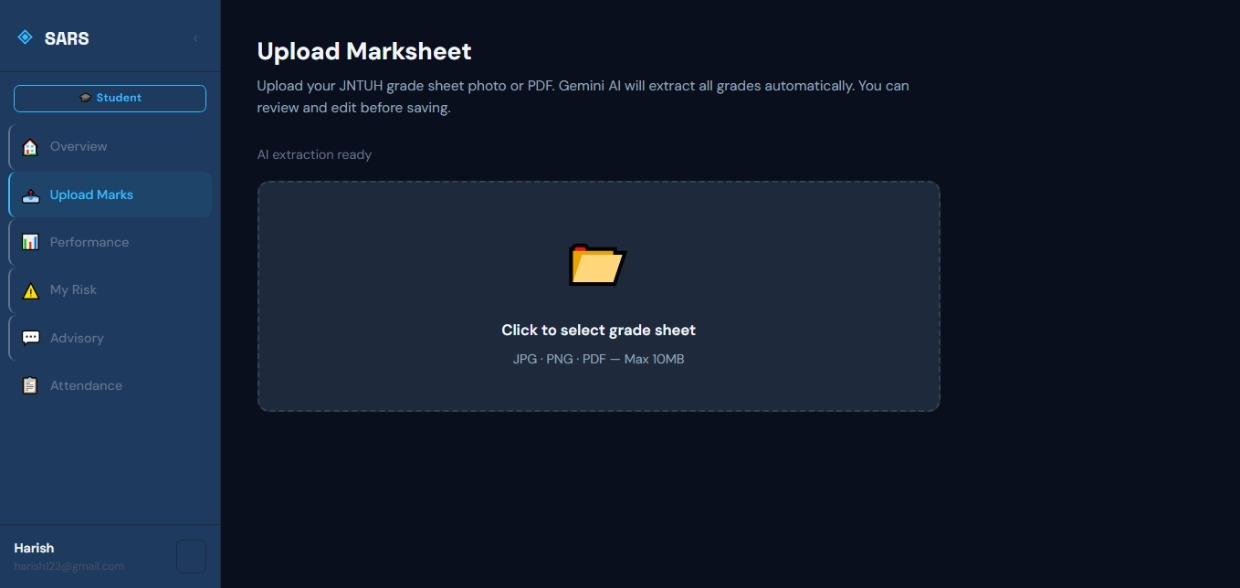
\includegraphics[width=0.48\linewidth]{upload_marksheet.jpeg}
    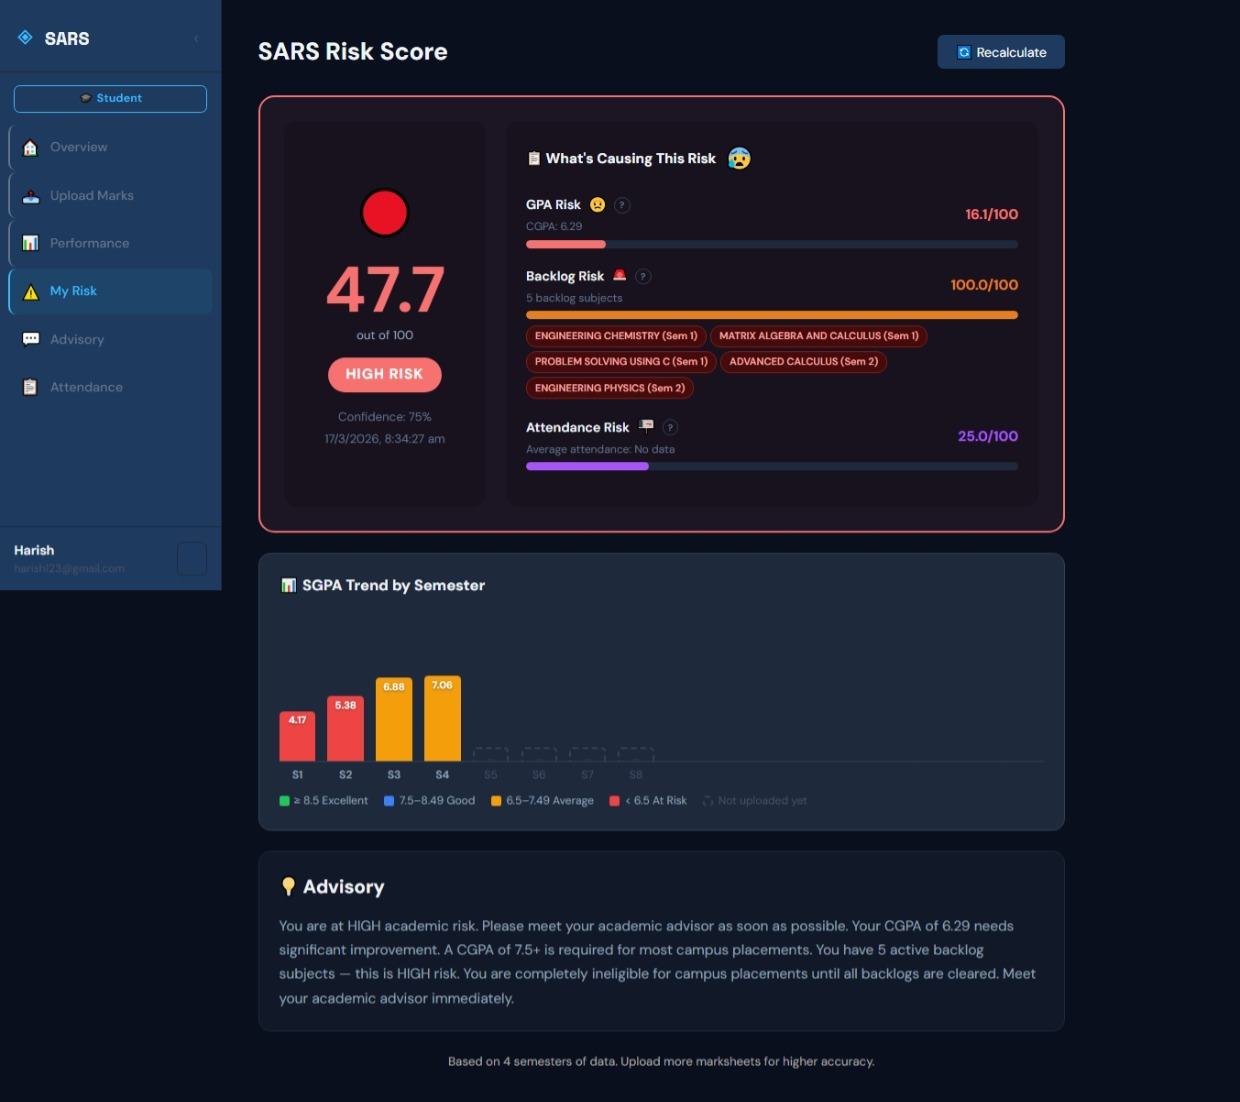
\includegraphics[width=0.48\linewidth]{risk_analysis_high.jpeg}

    \vspace{0.12cm}
    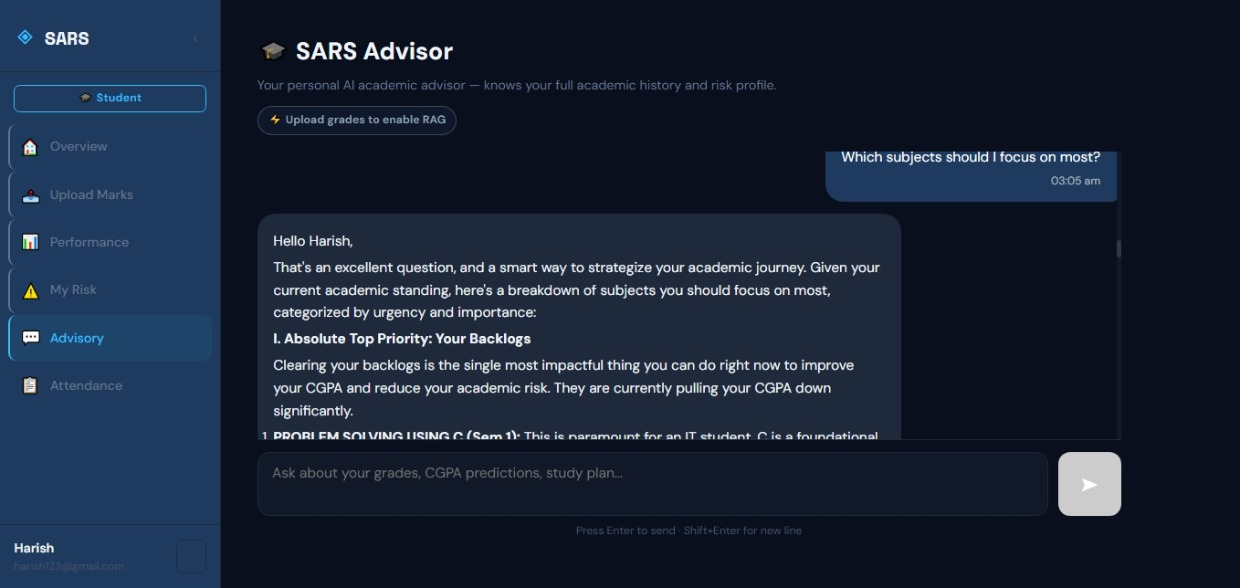
\includegraphics[width=0.48\linewidth]{advisory_high.jpeg}
    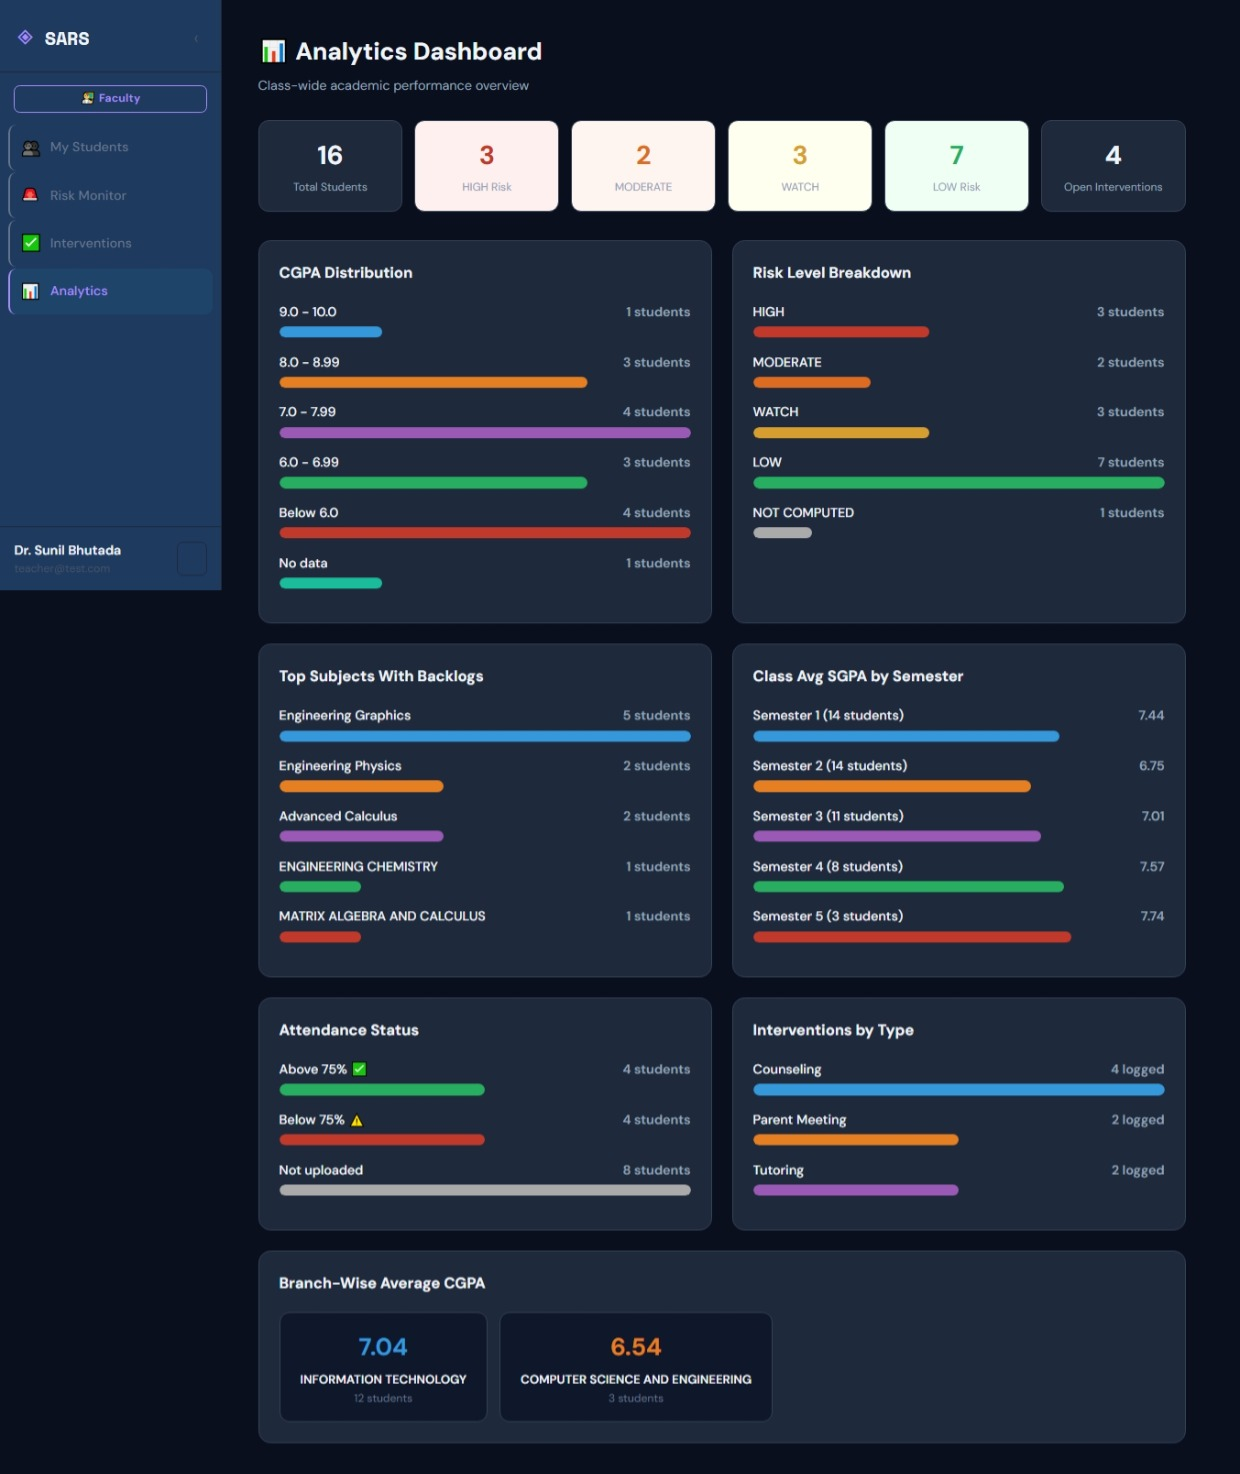
\includegraphics[width=0.48\linewidth]{teacher_analytics.jpeg}
  \end{columns}
\end{frame}

\begin{frame}{Advantages}
  \begin{itemize}
    \item Automates marksheet interpretation from PDF and image inputs
    \item Reduces manual workload for students and faculty advisors
    \item Provides explainable factor-wise academic risk assessment
    \item Grounds advisory responses in the student's own academic data
    \item Supports both self-monitoring and teacher-led intervention
    \item Uses a modular stack that is practical for pilot deployment
  \end{itemize}
\end{frame}

\begin{frame}{Limitations}
  \begin{itemize}
    \item Current evaluation is based on a limited project-scale dataset and screenshot-backed validation.
    \item OCR and extraction quality can vary with marksheet image quality and formatting differences.
    \item Risk thresholds may need recalibration for other institutions and policies.
    \item Large-scale live deployment and long-term field validation are still pending.
    \item Advisory quality depends on the completeness of stored academic evidence.
  \end{itemize}
\end{frame}

\begin{frame}{Conclusion}
  \begin{itemize}
    \item SARS integrates document ingestion, structured storage, explainable risk computation, and personalized advisory in a single academic workflow.
    \item The system demonstrates that educational analytics can be practical, transparent, and action-oriented.
    \item Student and teacher dashboards make academic risk visible and support timely intervention.
    \item The project establishes a strong foundation for explainable academic decision support in higher education.
  \end{itemize}
\end{frame}

\begin{frame}{Future Scope}
  \begin{itemize}
    \item Integration with institutional ERP or student information systems
    \item Automated alerts and early warning notifications
    \item Richer teacher analytics and department-level dashboards
    \item Multilingual advisory support for wider accessibility
    \item Improved OCR robustness across more grade sheet formats
    \item Larger-scale validation with real institutional datasets
  \end{itemize}
\end{frame}

\begin{frame}{References}
  \small
  \begin{enumerate}
    \item R. S. J. D. Baker and G. Siemens, ``Educational data mining and learning analytics,'' \textit{Learning Analytics}, 2014.
    \item S. M. Jayaprakash et al., ``Early alert of academically at-risk students,'' \textit{Journal of Learning Analytics}, 2014.
    \item H. Khosravi, S. Shum, and R. Chen, ``Explainable artificial intelligence in education,'' \textit{Computers and Education: Artificial Intelligence}, 2022.
    \item P. Lewis et al., ``Retrieval-augmented generation for knowledge-intensive NLP tasks,'' \textit{NeurIPS}, 2020.
    \item Y. Gao et al., ``Retrieval-augmented generation for large language models: A survey,'' arXiv, 2023.
  \end{enumerate}
\end{frame}

\begin{frame}[plain]
  \centering
  \vspace{1.4cm}
  {\usebeamercolor[fg]{title}\bfseries\LARGE Thank You}

  \vspace{0.5cm}
  {\large Questions and Discussion}

  \vspace{0.9cm}
  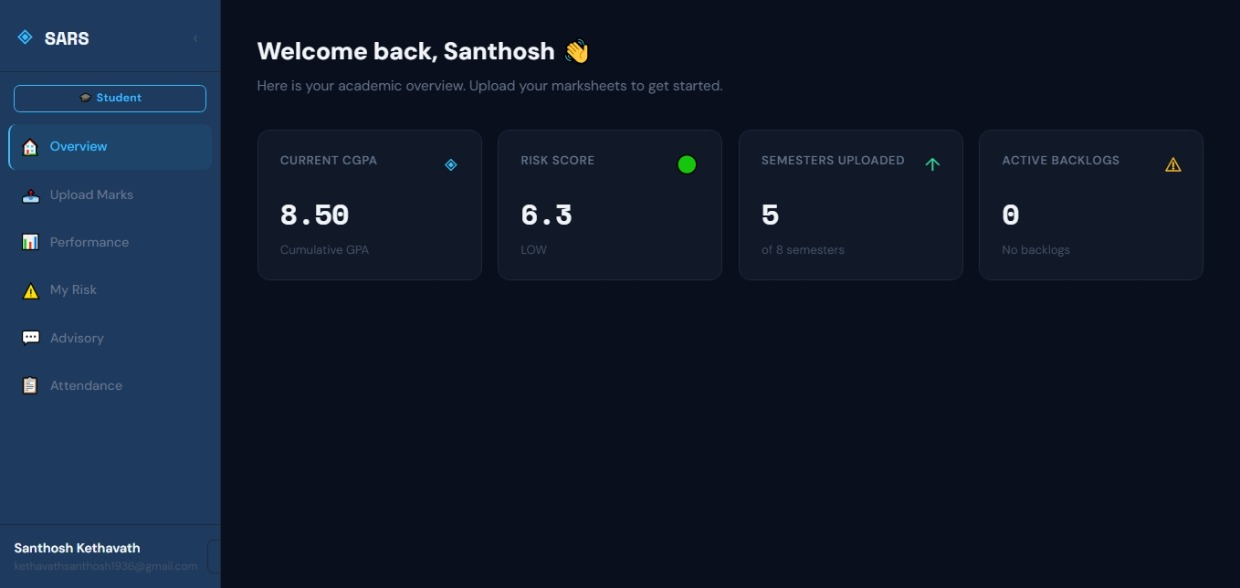
\includegraphics[width=0.56\linewidth,height=0.34\textheight,keepaspectratio]{student_dashboard_low.jpeg}
\end{frame}

\end{document}
